\documentclass[unicode,11pt,a4paper,oneside,numbers=endperiod,openany]{scrartcl}
\usepackage{graphicx}
\usepackage{subfig}
\usepackage{float}

\usepackage{ifthen}
\usepackage[utf8]{inputenc}
\usepackage{graphics}
\usepackage{graphicx}
\usepackage{hyperref}

\pagestyle{plain}
\voffset -5mm
\oddsidemargin  0mm
\evensidemargin -11mm
\marginparwidth 2cm
\marginparsep 0pt
\topmargin 0mm
\headheight 0pt
\headsep 0pt
\topskip 0pt        
\textheight 255mm
\textwidth 165mm

\newcommand{\duedate} {}
\newcommand{\setduedate}[1]{%
\renewcommand\duedate {Due date:~ #1}}
\newcommand\isassignment {false}
\newcommand{\setassignment}{\renewcommand\isassignment {true}}
\newcommand{\ifassignment}[1]{\ifthenelse{\boolean{\isassignment}}{#1}{}}
\newcommand{\ifnotassignment}[1]{\ifthenelse{\boolean{\isassignment}}{}{#1}}

\newcommand{\assignmentpolicy}{
\begin{table}[h]
\begin{center}
\scalebox{0.8} {%
\begin{tabular}{|p{0.02cm}p{16cm}|}
\hline
&\\
\multicolumn{2}{|c|}{\Large\textbf{HPC  2022 ---  Submission Instructions}}\\
\multicolumn{2}{|c|}{\large\textbf{(Please, notice that following instructions are mandatory: }}\\
\multicolumn{2}{|c|}{\large\textbf{submissions that don't comply with, won't be considered)}}\\
&\\
\textbullet & Assignments must be submitted to \href{https://www.icorsi.ch/course/view.php?id=14652}{iCorsi} (i.e. in electronic format).\\
\textbullet & Provide both executable package and sources (e.g. C/C++ files, Matlab). 
If you are using libraries, please add them in the file. Sources must be organized in directories called:\\
\multicolumn{2}{|c|}{\textit{Project\_number\_lastname\_firstname}}\\
& and  the  file must be called:\\
\multicolumn{2}{|c|}{\textit{project\_number\_lastname\_firstname.zip}}\\
\multicolumn{2}{|c|}{\textit{project\_number\_lastname\_firstname.pdf}}\\
\textbullet &  The TAs will grade your project by reviewing your project write-up, and looking at the implementation 
                 you attempted, and benchmarking your code's performance.\\

\textbullet & You are allowed to discuss all questions with anyone you like; however: (i) your submission must list anyone you discussed problems with and (ii) you must write up your submission independently.\\
\hline
\end{tabular}
}
\end{center}
\end{table}
}
\newcommand{\punkte}[1]{\hspace{1ex}\emph{\mdseries\hfill(#1~\ifcase#1{Points}\or{Points}\else{Points}\fi)}}


\newcommand\serieheader[6]{
\thispagestyle{empty}%
\begin{flushleft}

\includegraphics[width=0.4\textwidth]{usi_inf.png}
\end{flushleft}
  \noindent%
  {\large\ignorespaces{\textbf{#1}}\hspace{\fill}\ignorespaces{ \textbf{#2}}}\\ \\%
  {\large\ignorespaces #3 \hspace{\fill}\ignorespaces #4}\\
  \noindent%
  \bigskip
  \hrule\par\bigskip\noindent%
  \bigskip {\ignorespaces {\Large{\textbf{#5}}}
  \hspace{\fill}\ignorespaces \large \ifthenelse{\boolean{\isassignment}}{\duedate}{#6}}
  \hrule\par\bigskip\noindent%  \linebreak
 }

\makeatletter
\def\enumerateMod{\ifnum \@enumdepth >3 \@toodeep\else
      \advance\@enumdepth \@ne
      \edef\@enumctr{enum\romannumeral\the\@enumdepth}\list
      {\csname label\@enumctr\endcsname}{\usecounter
        {\@enumctr}%%%? the following differs from "enumerate"
	\topsep0pt%
	\partopsep0pt%
	\itemsep0pt%
	\def\makelabel##1{\hss\llap{##1}}}\fi}
\let\endenumerateMod =\endlist
\makeatother




\usepackage{textcomp}





\begin{document}


\setassignment
\setduedate{23.11.2022, 23:59}

\serieheader{High-Performance Computing}{2022}{Student: SIMONE TARENZI}{Discussed with: VEDANG NAIK, ISIN SU ECEVIT}{Solution for Project 4}{}
\newline


\section{Ring maximum using MPI [10 Points]}

First I used a simple way to get what rank the left and right neighbours of each node are.
\newline
The right node is given by the expression (my\_rank+1)\%size: in our case for example, node 3 will have as its right neighbour 0, because (3+1)\%4 is 0.
\newline
The left node instead is given by the expression (my\_rank-1+size)\%size, meaning that node 0 will have as its left neighbour node 3, since (0-1+4)\%4 = 3.
\newline
Implementing the actual comunication between nodes was pretty straightforward: each node, after making the operation to calculate its own max,  goes into the for loop in which it sends that max to its right neighbour, and receive the max of its left neighbour. If the max it receives is higher than its own, its max becomes the new max, and so it will send that to its right neighbour. At the end of the loop, each node will have the max between every node, which in our case is 6.

\section{Ghost cells exchange between neighboring processes [15 Points]}

This exercise was a bit trickier to understand. 
\newline
For starters, the documentation found online for the MPI\_Cart\_shift command was actually wrong, since it reversed how to find the left and right neighbours with the top and bottom ones.
\newline
After that, I had to create an additional MPI\_Datatype. I used the given data\_ghost for columns and created data\_row for rows.
\newline
Rows are easier to create: since the matrices are created left to right, top to bottom, the array of data will get the sequence of doubles as-is.
\newline
To create the columns instead,  it needs to jump 8 indices to get the next correct number (Fig.1).

\begin{figure}[H]
\centering
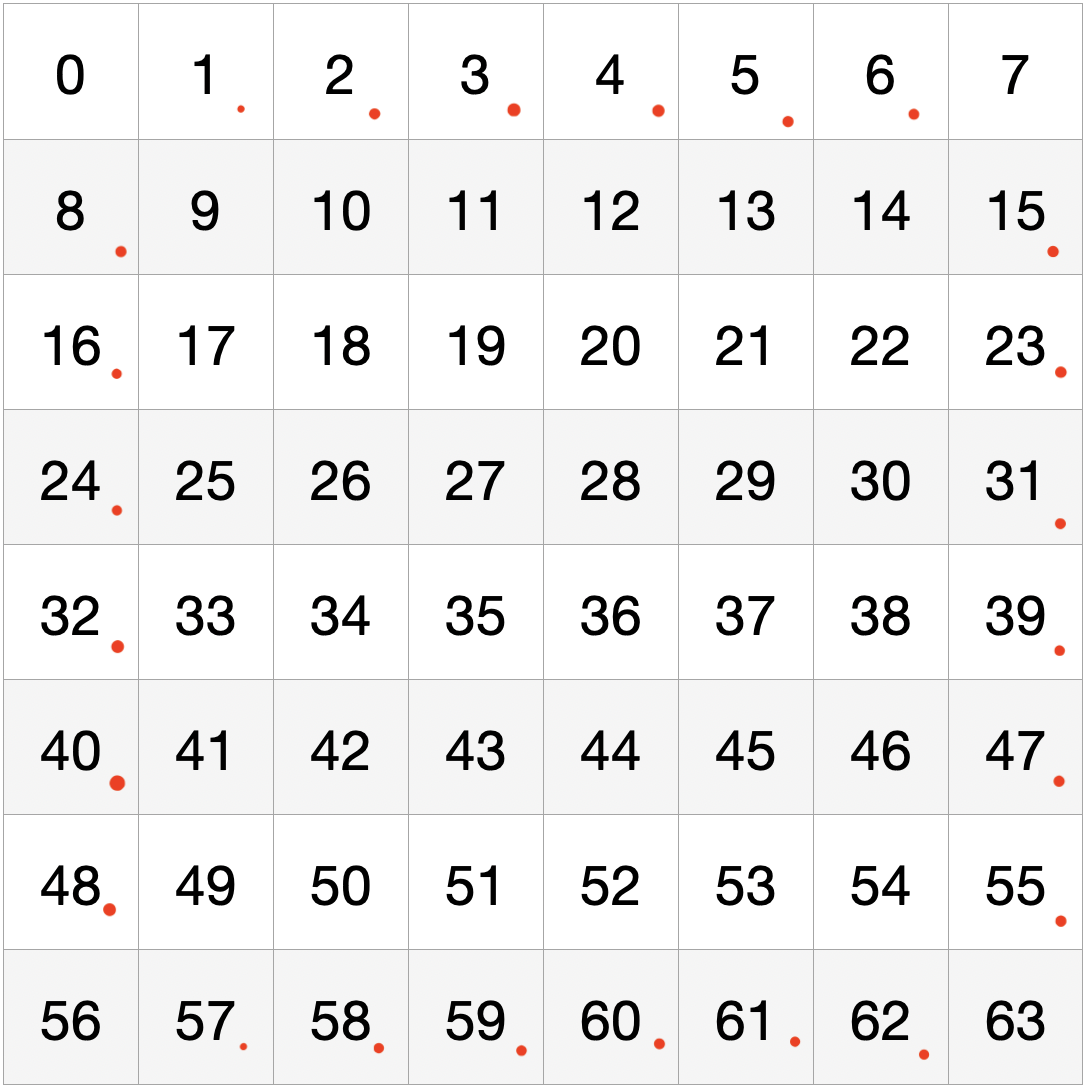
\includegraphics[width=0.5\linewidth]{ghost_matrix.png}
\caption{the ghost matrix indices, red dots represent the ones to send}
\end{figure}

After the datatypes are created, I can send them.
\newline
First I send all the data to the neighbours, and then it can be received. Trying to send only one vector at a time and receiving it immediately after creates unwanted results.
\newline
The code works with any of the processes, even boundary ones.

\section{Parallelizing the Mandelbrot set using MPI [20 Points]}

\begin{figure}[H]
\centering

\includegraphics[width=0.6\linewidth]{mandel.png}
\caption{the resulting mandelbrot image}
\end{figure}

\begin{figure}[H]
\centering
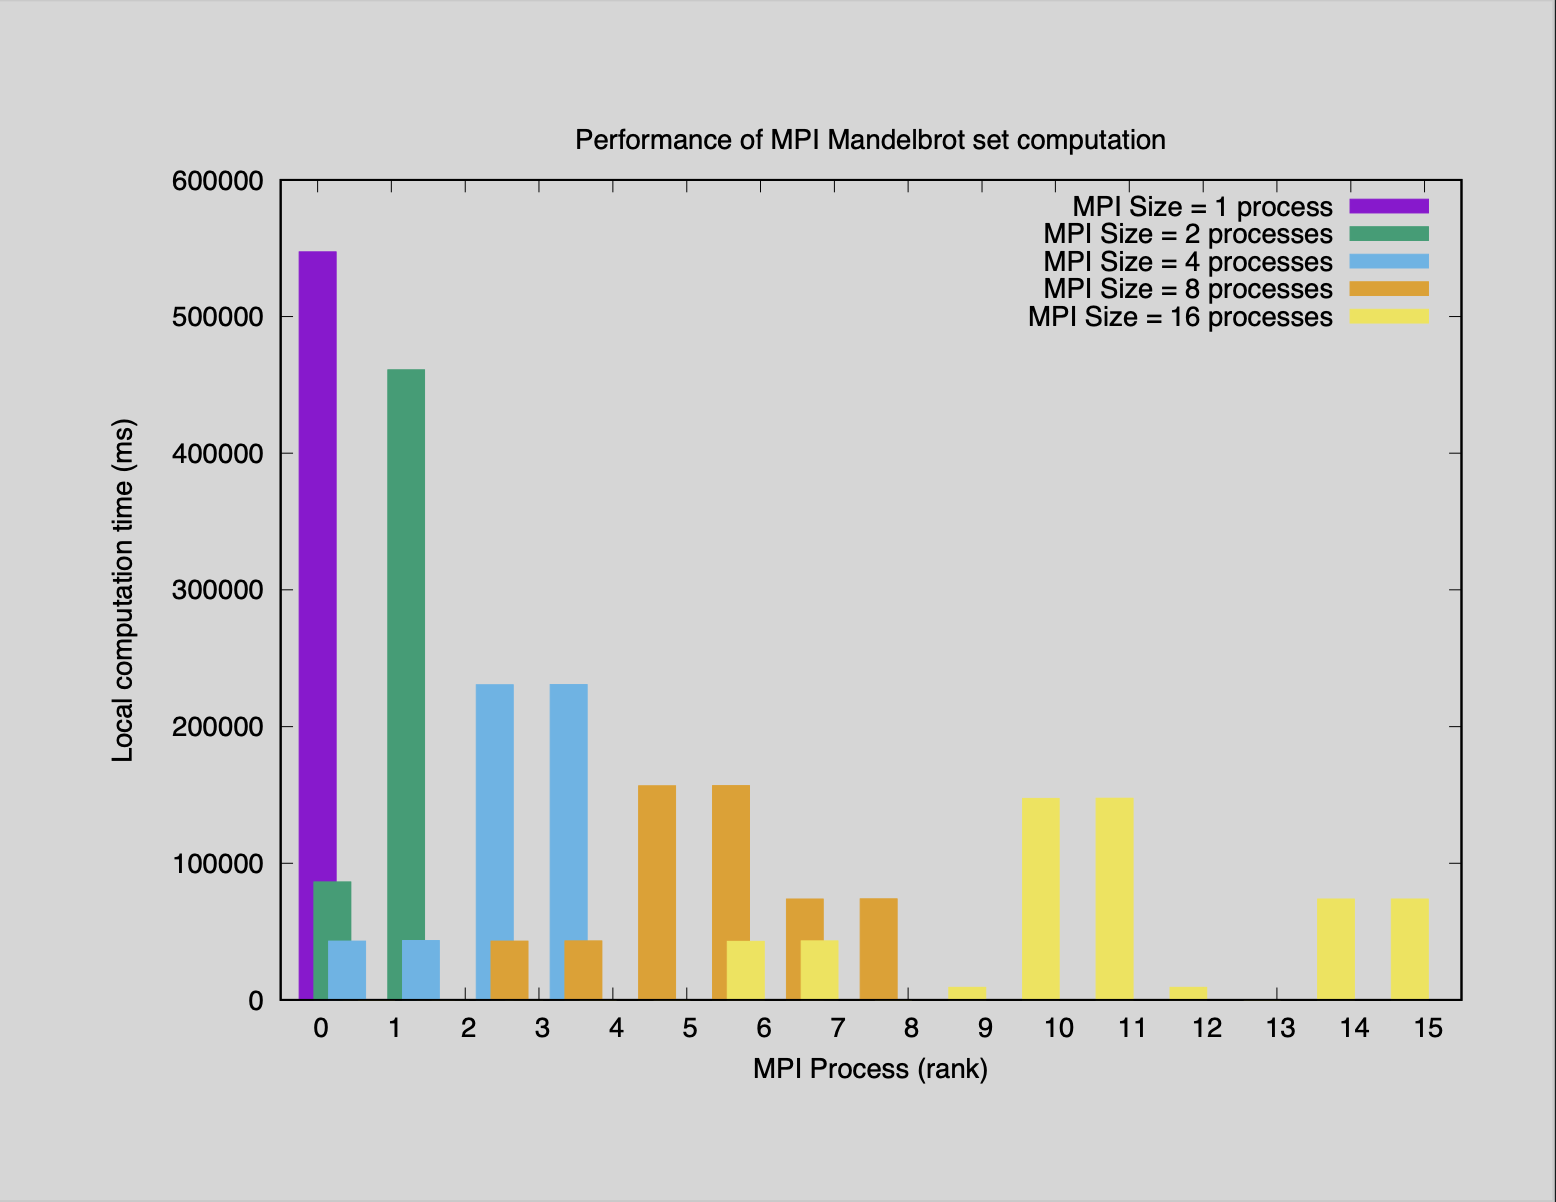
\includegraphics[width=0.6\linewidth]{perf.png}
\caption{the perf.ps performance graph of the computation divided between various number of processes}
\end{figure}

The performance is already improved when using 2 processes instead of one, but a really interesting finding is that the computation time isn't evenly distributed between the processes.


\section{Option A: Parallel matrix-vector multiplication and the power method [40 Points]}

I couldn't implement the parallelization, but the lambda result should at least be correct.

\section{Task:  Quality of the Report [15 Points]}

\end{document}
